%
\section{Model Training}
\label{sec:training}

A 3DMM consists of three parametric models: the \emph{shape},
\emph{camera} and \emph{texture} models.

%
%
%
\subsection{Shape Model}
Let us denote the 3D mesh (shape) of an object with $N$ vertexes as a
$3N\times 1$ vector
%
\begin{equation}
\mathbf{s} = {\left[\mathbf{x}_1^\mathsf{T}, \ldots, \mathbf{x}_N^\mathsf{T}\right]}^\mathsf{T} = {\left[x_1, y_1, z_1, \ldots, x_N, y_N, z_N\right]}^\mathsf{T}
\label{equ:3D_shape_vector}
\end{equation}
%
where $\mathbf{x}_i={\left[x_i, y_i, z_i\right]}^\mathsf{T}$ are the
object-centered Cartesian coordinates of the $i$-th vertex. A 3D shape model can be constructed by first bringing a set of 3D training meshes into dense correspondence so that each is described with the same number of vertexes and all samples have a shared semantic ordering.
The corresponded meshes, $\left\lbrace\mathbf{s}_i\right\rbrace$, are then brought into a shape space by applying Generalized Procrustes Analysis and then Principal Component Analysis (PCA) is performed which results in
$\left\lbrace\bar{\mathbf{s}}, \mathbf{U}_s\right\rbrace$, where
$\bar{\mathbf{s}}\in\mathbb{R}^{3N}$ is the mean shape vector and
$\mathbf{U}_s\in\mathbb{R}^{3N\times n_s}$ is the orthonormal basis after
keeping the first $n_s$ principal components. This model can be used to
generate novel 3D shape instances using the function
$\mathcal{S}: \mathbb{R}^{n_s} \rightarrow \mathbb{R}^{3N}$ as
%
\begin{equation}
\mathcal{S}(\mathbf{p}) = \bar{\mathbf{s}} + \mathbf{U}_s \mathbf{p}
\label{equ:shape_instance}
\end{equation}
%
where $\mathbf{p}={\left[p_1,\ldots,p_{n_s}\right]}^\mathsf{T}$ are the $n_s$ \emph{shape parameters}.


\begin{figure}[!t]
    \centering
    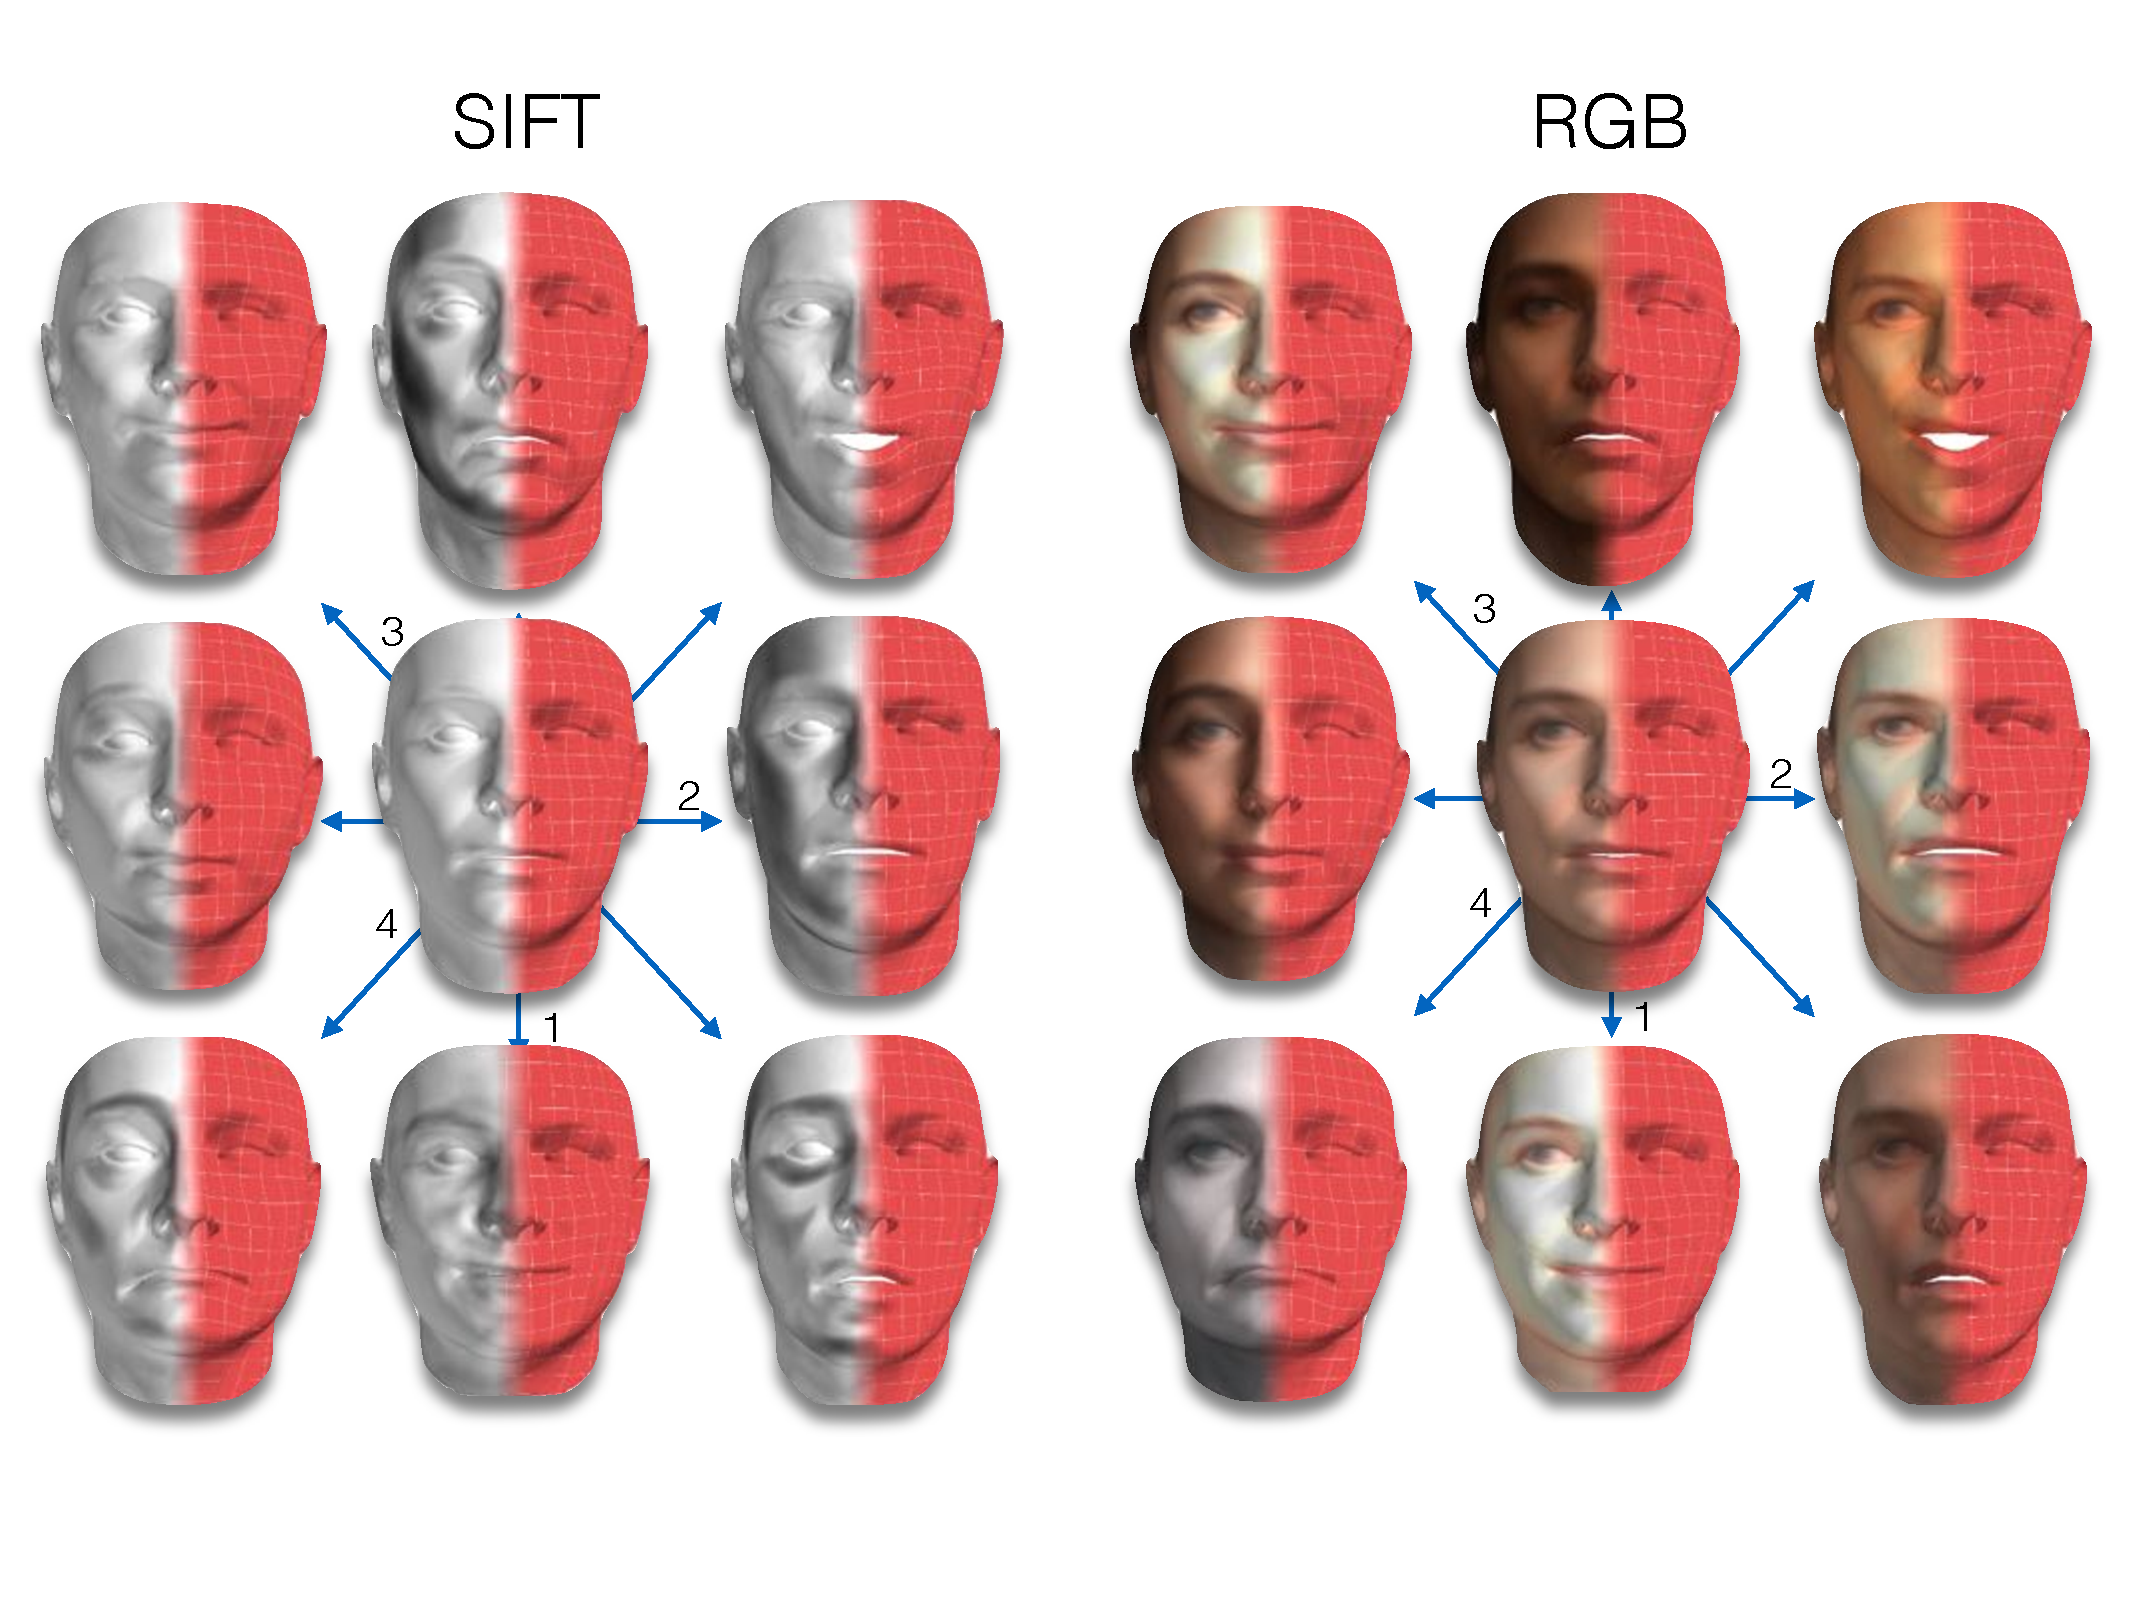
\includegraphics[width=\linewidth]{basis}
    \caption{\emph{Left:} The mean and first four shape and SIFT texture principal components of our ``in-the-wild'' SIFT texture model. \emph{Right:} To aid in interpretation we also show the equivalent RGB basis.}
\label{fig:basis}
\end{figure}
%
%
%
\subsection{Camera Model}
The purpose of the camera model is to map (project) the object-centered Cartesian
coordinates of a 3D mesh instance $\mathbf{s}$ into 2D Cartesian coordinates on
an image plane. In this work, we employ a pinhole camera model, which utilizes a
perspective transformation. However, an orthographic projection model can also
be used in the same way.

%
\textbf{Perspective projection.} The projection of a 3D point
$\mathbf{x}={[x,y,z]}^\mathsf{T}$ into its 2D location in the image plane
$\mathbf{x}'={[x',y']}^\mathsf{T}$ involves two steps. First, the 3D point is
rotated and translated using a linear \emph{view transformation}, under the
assumption that the camera is still
%
\begin{equation}
{\left[v_x, v_y, v_z\right]}^\mathsf{T} = \mathbf{R}_v\mathbf{x} + \mathbf{t}_v
\label{equ:view_transform}
\end{equation}
%
where $\mathbf{R}_v\in\mathbb{R}^{3\times 3}$ and
$\mathbf{t}_v={[t_x,t_y,t_z]}^\mathsf{T}$ are the 3D rotation and translation
components, respectively. Then, a non-linear \emph{perspective transformation}
is applied as
%
\begin{equation}
\mathbf{x}' = \frac{f}{v_z}\left[\begin{array}{c}v_x\\v_y\end{array}\right] + \left[\begin{array}{c}c_x\\c_y\end{array}\right]
\label{equ:perspective_transform}
\end{equation}
%
where $f$ is the focal length in pixel units (we assume that the $x$ and $y$ components of the focal length are equal) and
${[c_x, c_y]}^\mathsf{T}$ is the principal point that is set to the image center.

%
\textbf{Quaternions.}
We parametrize the 3D rotation with quaternions~\cite{kuipers1999quaternions,wheeler1995iterative}.
The quaternion uses four parameters
$\mathbf{q}={\left[q_0,q_1,q_2,q_3\right]}^\mathsf{T}$ in order to express a 3D
rotation as
%
\begin{equation}
\mathbf{R}_v =
2\left[\begin{array}{ccc}
\frac{1}{2}-q_2^2-q_3^2 & q_1q_2-q_0q_3 & q_1q_3+q_0q_2\\
q_1q_2+q_0q_3 & \frac{1}{2}-q_1^2-q_3^2 & q_2q_3-q_0q_1\\
q_1q_3-q_0q_2 & q_2q_3+q_0q_1 & \frac{1}{2}-q_1^2-q_2^2
\end{array}\right]
\end{equation}
%
Note that by enforcing a unit norm constraint on the quaternion vector, i.e.
$\mathbf{q}^\mathsf{T}\mathbf{q}=1$, the rotation matrix constraints of
orthogonality with unit determinant are withheld. Given the unit norm property,
the quaternion can be seen as a three-parameter vector
${\left[q_1,q_2,q_3\right]}^\mathsf{T}$ and a scalar
$q_0=\sqrt{1-q_1^2-q_2^2-q_3^2}$. Most existing works on 3DMM parametrize the
rotation matrix $\mathbf{R}_v$ using the three Euler angles that define the
rotations around the horizontal, vertical and camera axes. Even thought Euler
angles are more naturally interpretable, they have strong disadvantages when
employed within an optimization procedure, most notably the solution ambiguity
and the gimbal lock effect. Parametrization based on quaternions overcomes these
disadvantages and further ensures computational efficiency, robustness and
simpler differentiation.

%
\textbf{Camera function.}
The projection operation performed by the camera model of the 3DMM can be
expressed with the function
$\mathcal{P}(\mathbf{s},\mathbf{c}): \mathbb{R}^{3N} \rightarrow \mathbb{R}^{2N}$,
which applies the transformations of Eqs.~\ref{equ:view_transform} and~\ref{equ:perspective_transform}
on the points of provided 3D mesh $\mathbf{s}$ with
%
\begin{equation}
\mathbf{c} = {\left[f, q_1, q_2, q_3, t_x, t_y, t_z\right]}^\mathsf{T}
\end{equation}
%
being the vector of \emph{camera parameters} with length $n_c=7$.
For abbreviation purposes, we represent the camera model of the 3DMM with the
function $\mathcal{W}: \mathbb{R}^{n_s,n_c} \rightarrow \mathbb{R}^{2N}$ as
%
\begin{equation}
\mathcal{W}(\mathbf{p},\mathbf{c})\equiv\mathcal{P}\left(\mathcal{S}(\mathbf{p}),\mathbf{c}\right)
\label{equ:camera_model}
\end{equation}
%
where $\mathcal{S}(\mathbf{p})$ is a 3D mesh instance using Eq.~\ref{equ:shape_instance}.

%
%
%
\subsection{``In-the-Wild'' Feature-Based Texture Model}
\label{sec:texture-model}
The generation of an ``in-the-wild'' texture model is a key component of the
proposed 3DMM. To this end, we take advantage of the existing large facial ``in-the-wild''
databases that are annotated in terms of sparse landmarks.
Assume that for a set of $M$ ``in-the-wild'' images
$\left\lbrace\mathbf{I}_i\right\rbrace_1^M$, we have access to the associated
camera and shape parameters $\left\lbrace\mathbf{p_i}, \mathbf{c_i}\right\rbrace$.
Let us also define a \emph{dense} feature extraction function
%
\begin{equation}
\mathcal{F}: \mathbb{R}^{H\times W}\rightarrow\mathbb{R}^{H\times W \times C}
\label{equ:features}
\end{equation}
%
where $C$ is the number of channels of the feature-based image. For each image,
we first compute its feature-based representation as
$\mathbf{F}_i = \mathcal{F}(\mathbf{I}_i)$ and then use Eq.~\ref{equ:camera_model}
to sample it at each vertex location to build back a vectorized texture sample
$\mathbf{t}_i = \mathbf{F}_i\left(\mathcal{W}(\mathbf{p_i},\mathbf{c_i})\right) \in \mathbb{R}^{CN}$.
This texture sample will be nonsensical for some regions mainly due to self-occlusions
present in the mesh projected in the image space
$\mathcal{W}(\mathbf{p_i},\mathbf{c_i})$.
%
To alleviate these issues, we cast a ray from the camera to each vertex and test
for self-intersections with the triangulation of the mesh in order to learn a
per-vertex occlusion mask $\mathbf{m}_i\in\mathbb{R}^{N}$ for the projected sample.

Let us create the matrix
$\mathbf{X}=\left[\mathbf{t}_1, \ldots, \mathbf{t}_M\right]\in\mathbb{R}^{CN \times M}$
by concatenating the $M$ grossly corrupted feature-based texture vectors with missing entries that are represented by the masks $\mathbf{m}_i$.
To robustly build a texture model based on this heavily contaminated incomplete
data, we need to recover a low-rank matrix $\mathbf{L}\in\mathbb{R}^{CN \times M}$
representing the clean facial texture and a sparse matrix $\mathbf{E}\in\mathbb{R}^{CN \times M}$
accounting for gross but sparse non-Gaussian noise such that $\mathbf{X}=\mathbf{L}+\mathbf{E}$.
To simultaneously recover both $\mathbf{L}$ and $\mathbf{E}$ from incomplete and
grossly corrupted observations, the Principal Component Pursuit with missing
values~\cite{shang2014robust} is solved
%
\begin{equation}
\begin{aligned}
\argmin_{\mathbf{L},\mathbf{E}} &~\lVert\mathbf{L}\rVert_* + \lambda \lVert\mathbf{E}\rVert_1\\
\mbox{s.t.} &~\mathcal{P}_{\Omega}( \mathbf{X}) = \mathcal{P}_{\Omega}( \mathbf{L} +  \mathbf{E}),
\label{E:PCP}
\end{aligned}
\end{equation}
%
where $\lVert\cdot\rVert_*$ denotes the nuclear norm,
$\lVert\cdot\rVert_1$ is the matrix $\ell_1$-norm and $\lambda>0$ is a regularizer.
$\Omega$ represents the set of locations corresponding to the observed entries
of $\mathbf{X}$ (i.e., $(i,j)\in\Omega~\text{if}~m_i=m_j=1$). Then,
$\mathcal{P}_{\Omega}(\mathbf{X})$ is defined as the projection of the matrix
$\mathbf{X}$ on the observed entries $\Omega$, namely
${\mathcal{P}_{\Omega}(\mathbf{X})}_{ij} = x_{ij}~\text{if}~(i,j)\in\Omega$
and ${\mathcal{P}_{\Omega}(\mathbf{X})}_{ij}=0$ otherwise.
The unique solution of the convex optimization problem in Eq.~\ref{E:PCP} is found by employing an Alternating Direction Method of Multipliers-based algorithm~\cite{bertsekas2014constrained}.

\begin{figure}[!t]
    \centering
    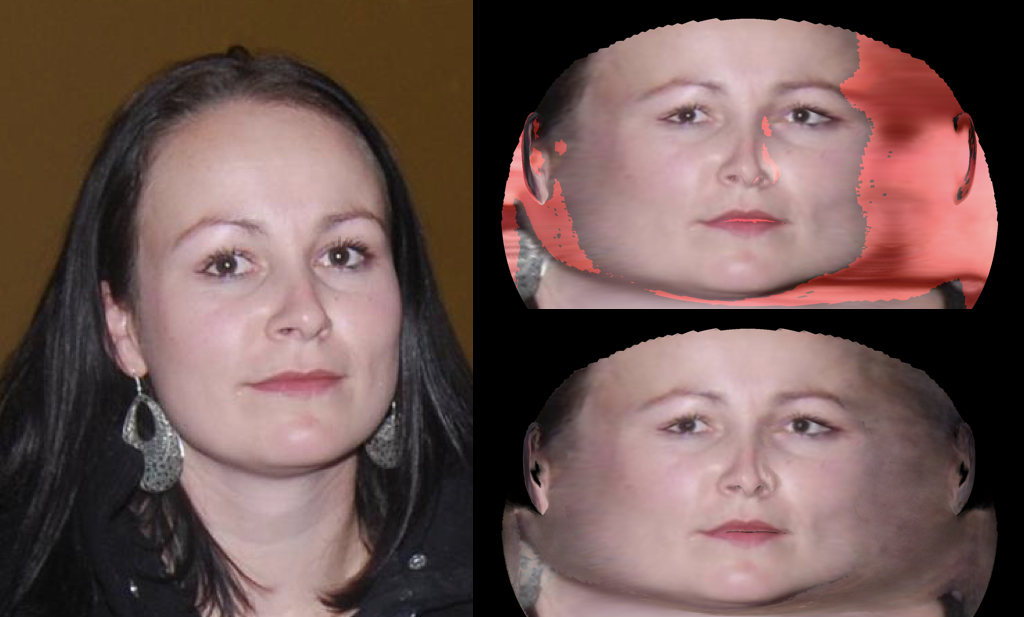
\includegraphics[width=0.7\linewidth]{itw_extraction}
    \caption{Building an ITW texture model}
\label{fig:itw_extraction}
\end{figure}
The final texture model is created by applying PCA on the set of reconstructed
feature-based textures acquired from the previous procedure. This results in
$\left\lbrace\bar{\mathbf{t}}, \mathbf{U}_t\right\rbrace$,
where $\bar{\mathbf{t}}\in\mathbb{R}^{CN}$ is the mean texture vector and
$\mathbf{U}_t\in\mathbb{R}^{CN\times n_t}$ is the orthonormal basis after
keeping the first $n_t$ principal components. This model can be used to generate
novel 3D feature-based texture instances with the function
$\mathcal{T}: \mathbb{R}^{n_t} \rightarrow \mathbb{R}^{CN}$ as
%
\begin{equation}
\mathcal{T}(\boldsymbol{\lambda}) = \bar{\mathbf{t}} + \mathbf{U}_t \boldsymbol{\lambda}
\label{equ:texture_instance}
\end{equation}
%
where $\boldsymbol{\lambda}={[\lambda_1,\ldots,\lambda_{n_t}]}^\mathsf{T}$ are the $n_t$ \emph{texture parameters}.

Finally, an iterative procedure is used in order to refine the texture. That is, we started with the 3D fits provided by using only the 2D landmarks \cite{jourabloo2016large}. Then, a texture model is learned using the above procedure. The texture model was used with the proposed 3DMM fitting algorithm on the same data and texture model was refined.
